\documentclass[10pt]{article}
\usepackage{../local}


\newcommand{\classcode}{Physics 110A}
\newcommand{\classname}{Electrodynamics and Optics}
\renewcommand{\maketitle}{%
\hrule height4pt
\large{Eric Du \hfill \classcode}
\newline
\large{HW 06} \Large{\hfill \classname \hfill} \large{\today}
\hrule height4pt \vskip .7em
\normalsize
}
\linespread{1.1}
\begin{document}
	\maketitle
	\section*{Collaborators}

	I worked with \textbf{Andrew Binder, Christine Zhang, Teja Nivarthi, Nathan Song} and \textbf{Nikhil 
	Maserang} to complete this assignment.

	\section*{Problem 1}
	A hollow cube has six square faces. Five faces are grounded $(V = 0)$, while the top face is held at a 
	constant potential $V = V_0$. Find the potential at the center of the cube. \textit{Hint:} Duplicate five 
	other such cubes. And then use the superposition principle. 

	\begin{center}
		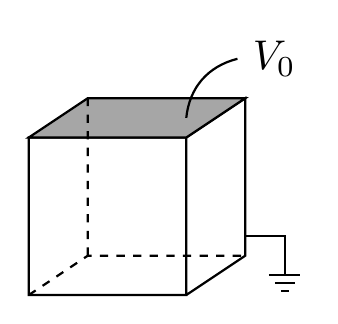
\begin{tikzpicture}
            \draw[thick] (0,0) -- (2,0) -- (2,2) -- (0,2) -- cycle (2,0) -- (2.75,0.5) -- (2.75,2.5) -- (2,2);
            \draw[thick, fill=gray!70] (0,2) -- (2,2) -- (2.75,2.5) -- (0.75,2.5) -- cycle;
            \draw[thick, dashed] (0,0) -- (0.75,0.5) -- (2.75,0.5) (0.75,0.5) -- (0.75,2.5);
            \draw[thick] (2,2.25) to[bend left=35] (2.65,3) node[anchor=west,scale=1.5] {$V_0$};
            \draw[thick] (2.75,0.75) -- (3.25,0.75) -- (3.25,0.25);
            \draw[thick] (3.05,0.25) -- (3.45,0.25)
                         (3.125,0.15) -- (3.375,0.15)
                         (3.2,0.05) -- (3.3,0.05);
        \end{tikzpicture}
	\end{center}
	\begin{solution}
		Following the hint, construct a cube with all five sides with potential $V_0$. Since there is no charge
		inside the cube, then it is impossible for there to be any electric field present. Now, since $\vec E = 
		-\nabla V$, then the condition that $\vec E = 0$ everywhere in the cube requires that there is no
		gradient within the cube, or in other words $V = V_0$ everywhere inside the cube. Therefore, $V = V_0$
		in the center of the cube as well. 

		Now, we can use the superposition principle. We expect that every plate contributes equally to the 
		potential at the center of the cube because the cube has rotational symmetry. Therefore, we conclude
		that the contribution of potential due to a single plate (which is also the potential the problem 
		statement asks us to find) is $V = \frac{V_0}{6}$.

		Alternatively, one could solve Laplace's equation with $\laplace V = 0$ and fit the boundary conditions,
		but that approach is longer, and I frankly find this one to be much cleaner and more conceptual. 
	\end{solution}

	\pagebreak 
	\section*{Problem 2}
	A sphere centered at the origin has radius $R$. The electric field within the sphere is given by
	\[
	E = -\frac{V_0x}{R^2}\hat{x} - \frac{V_0y}{R^2}\hat{y} + \frac{2V_0z}{R^2}\hat{z}\ \ \text{for $x^2 + y^2
	+z^2 \le R^2$}
	\] 
	Find the volume charge density $\rho(r, \theta, \phi)$ (confined to $r < R$) and the surface charge density
	$\sigma(\theta)$ (confined to $r = R$) that produce the electric field given above. We assume there is no 
	charge outside the sphere for this problem. Express your answer in terms of spherical coordinates. Is
	your answer unique? If not, find the general charge distributions that produce such electric field. 

	\begin{solution}
		First, we can find the volumetric charge density by taking the divergence of this vector field. We can 
		take it in cartesian coordinates since our choice of coordinate system here really doesn't matter. Doing
		this, we find:
		\[
		\div E = -\frac{V_0}{R^2}\left( 0 + 0 + 0\right) = 0 = \frac{\rho(x, y, z)}{\epsilon_0}
		\] 
		So this means that $\rho(x, y, z) = 0$. This also implies that $\rho(r, \theta, \phi) = 0$, since 
		changing the coordinate system does not change the volume we're interested in. To find the surface
		charge density, we first note that the general solution to the potential is:
		\[
			V(r, \theta) = \sum_{l = 0}^\infty \left( A_l r^l + \frac{B_l}{r^{l+1}} \right) P_l(\cos \theta)
		\] 
		Outside, we know that there are no charges so the potential should equal 0 at infinity, meaning that 
		outside, the potential is: 
		\[
			V_{out}(r, \theta) = \sum_{l = 0}^\infty \frac{B_l}{r^{l+1}} P_l(\cos \theta)
		\]
		To find the potential inside the sphere, notice that we're given the electric field, so using $E = 
		-\nabla V$ and a little bit of algebra we find that:
		\[
			V_{in}(r, \theta) = \frac{V_0}{R^2}\left( \frac{x^2}{2} + \frac{y^2}{2} - z^2 \right) 
		\] 
		So now using the substitution that $x = r\sin \theta \sin \phi, y = r \sin \theta \sin \phi, z = r \cos
		\theta$, then we get:
		\begin{align*}
			V_{in}(r, \theta) &= \frac{V_0}{R^2}\left( \frac{r^2 \sin^2 \theta \cos^2 \phi}{2} + 
			\frac{r^2 \sin^2 \theta \sin^2 \phi}{2} - r^2 \cos^2 \theta \right)  \\
			&= \frac{V_0r^2}{R^2}\left( \frac{\sin^2 \theta}{2} - \cos^2 \theta \right)  \\
			&= \frac{V_0r^2}{2R^2}(1 - 3\cos^2 \theta)
		\end{align*}
		Evaluating this expression at $R$ gives:
		\[
		 V(r = R, \theta) = \frac{V_0}{2}(1 - 3 \cos^2 \theta) = -\frac{V_0}{2}P_2(\cos \theta)
		\] 
		where $P_2$ represents the second Legendre polynomial. Outside the sphere, we have: 
		\[
			V_{out} (R, \theta) = \sum_{l = 0}^\infty \frac{B_l}{R^{l+1}}P_l(\cos \theta)
		\] 
		Since the Legendre polynomials are orthogonal to one another, this means that only the $l =2$ term 
		survives here, so we have $V_{out} = \dfrac{B_2}{R^3}P_2(\cos \theta)$. Now, we can equate the two 
		together: 
		\begin{align*}
			V_0 \cdot -P_2(\cos \theta) &= \frac{B_2}{R^3}P_2(\cos \theta)\\
			\therefore B_2 &=  -V_0R^3
		\end{align*}
		Therefore, 
		\[
			V_{out}(r, \theta) = -\frac{V_0R^3}{2r^3}(3 \cos^2 \theta -1)
		\] 
		Now we can proceed and find the surface charge density, using the relation that 
		\[ 
			\pdv{V}{r}\bigg|_{\text{below}}^{\text{above}} = -\frac{\sigma}{\epsilon_0}
		\] 	
		So calculating this:
		\begin{align*}
			\pdv{V_{out}}{r} - \pdv{V_{in}}{r} &= \left( -\frac{V_0R^3}{2} \cdot -\frac{3}{r^4} \right) 
			(3\cos^2 \theta - 1) - \left(\frac{2V_0r}{2R^2}(1 - 3\cos^2 \theta)\right)\\
			&= \frac{3V_0}{2R} (3\cos^2 \theta - 1) - \frac{V_0}{R}(1 - 3\cos^2 \theta)\\
			&= \frac{5V_0}{R}P_2(\cos \theta) = \frac{\sigma}{\epsilon_0} \\
			\therefore \sigma(\theta) &= \frac{5\epsilon_0V_0}{R}P_2(\cos \theta)
		\end{align*}
	\end{solution}
	\pagebreak

	\section*{Problem 3}
	Consider a capacitor formed by an infinitely large plate on $z = 0$ with $V = 0$, and an infinite, solid, 
	conducting cone with an interior angle $\pi/4$ held at potential $V = V_0$. Note that the tip of the cone 
	vertex and the infinitely large plate are insulated. 
	

	\begin{center}
		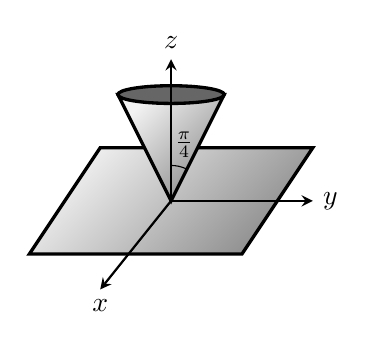
\begin{tikzpicture}[scale=0.9]
            \draw[very thick, shading=axis, left color=gray!90, right color=gray!10!white, shading angle=-135, anchor=south] (2,0.75) -- (-1,0.75) -- (-2,-0.75) -- (1,-0.75) -- cycle;
            \draw[very thick, shading=axis, left color=gray!90, right color=gray!10!white, shading angle=-135, anchor=south] (0.75,1.5) -- (0,0) -- (-0.75,1.5) -- cycle;
            \draw[very thick,fill=gray!120] (0,1.5) ellipse (0.75cm and 0.125cm);
            \draw[thick, -stealth] (0,0) -- (0,2) node[anchor=south] {$z$};
            \draw[thick, -stealth] (0,0) -- (2,0) node[anchor=west] {$y$};
            \draw[thick, -stealth] (0,0) -- (-1,-1.25) node[anchor=north] {$x$};
            \draw (0,0.5) arc (90:65:0.5cm) node[midway,above,scale=0.9,xshift=0.075cm] {$\frac{\pi}{4}$};
        \end{tikzpicture}
	\end{center}
	\begin{enumerate}[label=\alph*)]
		\item Based on symmetries, explain why $V(r, \theta, \phi) = V(\theta)$ in the space between the cone
			and the plate. (Note that here only the potential has this scale invariance. Other quantities such
			as the electric field and charge density do not.)

			\begin{solution}
				Firstly, there is rotational symmetry in the $\phi$ direction, so there can't be any $\phi$ 
				dependence. Furthermore, since there is no characteristic length scale of the system, there
				also cannot be any $r$ dependence. Therefore, $V$ can only depend on $\theta$.
			\end{solution}
		\item Integrate Laplace's equation explicitly to find the potential between the cone and the plate. (Note
			that the general solution Eq. (3.65) in Griffiths does not apply to the case here, since we have
			charges, distributed at $\theta = \pi/4$ and $\pi/2$.
			
			\begin{solution}
				We know that $\laplace V = 0$, so using spherical coordinates, this implies:
				\[
					\frac{1}{r^2\sin \theta} \pdv{\theta}\left( \sin \theta \pdv{V}{\theta} \right) = 0
				\] 
				So this implies that $\sin \theta \pdv{V}{\theta}$ is a constant, so integrating this: 
				\begin{align*}
					\sin \theta \pdv{V}{\theta} &= k \\
					\int dV &= \int \frac{k}{\sin \theta}d\theta  \\
					\therefore V(\theta) &= k\left( \ln\left( \sin \frac{\theta}{2} \right) -
					\ln\cos \frac{\theta}{2} \right) +C \\
					&= k\ln\left( \tan \frac{\theta}{2} \right) +C
				\end{align*}
				Substituting in $V(\frac{\pi}{2}) = 0$ gives us $C = 0$, and substituting $\theta =
				\frac{\pi}{2}$ gives:
				\begin{align*}
					k\log(\sqrt{2} -1) &= V_0 \\
					\therefore k&= \frac{V_0}{\ln(\sqrt{2} -1)}
				\end{align*}
				Finally, we get the full expression for $V(\theta)$: 
				\[
				V(\theta) = \frac{V_0}{\ln(\sqrt{2} -1)}\ln \left( \tan \frac{\theta}{2} \right) 
				\] 
			\end{solution}
	\end{enumerate}
\end{document}
